\documentclass[a4paper,14pt,russian]{extreport}
 \usepackage{extsizes}
%\usepackage{cmap} % для кодировки шрифтов в pdf<br/> 
 \usepackage[T2A]{fontenc}
 \usepackage[utf8]{inputenc}
\usepackage[ukrainian,russian]{babel}
\usepackage{listings}  
\lstset{language=Python}
%\usepackage{pscyr}
\usepackage{graphicx} % для вставки картинок<br/> 
\graphicspath{ {images/} }
\usepackage{amssymb,amsfonts,amsmath,amsthm} % математические дополнения от АМС<br/>
\usepackage{amsmath} 
\usepackage{indentfirst} % отделять первую строку раздела абзацным отступом тоже<br/> 
\usepackage[usenames,dvipsnames]{color} % названия цветов<br/>
\usepackage{makecell}
\usepackage{multirow} % улучшенное форматирование таблиц<br/> 
\usepackage{ulem} % подчеркивания<br/>  <br/> 
\linespread{1.3} % полуторный интервал<br/> 
\renewcommand{\rmdefault}{ftm} % Times New Roman<br/> 
\frenchspacing

%номерація в верхньому правому
\usepackage{fancyhdr} 
\pagestyle{fancy} 
\fancyhf{}
\fancyhead[R]{\thepage}
\fancyheadoffset{0mm} 
\fancyfootoffset{0mm} 
\setlength{\headheight}{17pt} 
\renewcommand{\headrulewidth}{0pt} 
\renewcommand{\footrulewidth}{0pt} 
\fancypagestyle{plain}{\fancyhf{}\rhead{\thepage}} 
\setcounter{page}{2} % начать нумерацию страниц с №5

 
%заголовки
 \usepackage{titlesec}
 \titleformat{\chapter}[display]
 {\filcenter}
 {\MakeUppercase{\chaptertitlename} \thechapter}
 {8pt}
 {\bfseries}{}
 \titleformat{\section}
 {\normalsize\bfseries}
 {\thesection}
 {1em}{}
 \titleformat{\subsection}
 {\normalsize\bfseries}
 {\thesubsection}
 {1em}{}
  % Настройка вертикальных и горизонтальных отступов<br/> 
 \titlespacing*{\chapter}{0pt}{-30pt}{8pt}
\titlespacing*{\section}{\parindent}{*4}{*4}
\titlespacing*{\subsection}{\parindent}{*4}{*4} 
 
 %відступи
 \usepackage{geometry} 
 \geometry{left=3cm}
 \geometry{right=1.5cm}
 \geometry{top=2.4cm}
 \geometry{bottom=2.4cm}
 
 %
\usepackage{tocloft}
\renewcommand{\cfttoctitlefont}{\hspace{0.38\textwidth} \bfseries\MakeUppercase}
\renewcommand{\cftbeforetoctitleskip}{-1em}
\renewcommand{\cftaftertoctitle}{\mbox{}\hfill \\ \mbox{}\hfill{\footnotesize Стр.}\vspace{-2.5em}}
\renewcommand{\cftchapfont}{\normalsize\bfseries \MakeUppercase{\chaptername} }
\renewcommand{\cftsecfont}{\hspace{31pt}}
\renewcommand{\cftsubsecfont}{\hspace{11pt}}
\renewcommand{\cftbeforechapskip}{1em}
\renewcommand{\cftparskip}{-1mm}
\renewcommand{\cftdotsep}{1}
\setcounter{tocdepth}{2} % задать глубину оглавления — до subsection включительно

\newcommand{\empline}{\mbox{}\newline}
\newcommand{\likechapterheading}[1]{
\begin{center}
     \textbf{\MakeUppercase{#1}}
     \end{center}
         \empline}
         
\makeatletter
\renewcommand{\@dotsep}{2}
\newcommand{\l@likechapter}[2]{{\bfseries\@dottedtocline{0}{0pt}{0pt}{#1}{#2}}}
\makeatother
\newcommand{\likechapter}[1]{
\likechapterheading{#1}
\addcontentsline{toc}{likechapter}{\MakeUppercase{#1}}}



\begin{document} 

\newpage
\tableofcontents
\newpage

\likechapter{Вступ}
Аналіз даних на сьогоднішній день лежить в основі багатьох прикладних програм та сервісів. Кластерний аналіз допомагає згрупувати інформацію за спільними ознаками. Інтуєтивно зрозуміло, що об'єкти з одного кластеру мають більшу міру схожості ніж з об'єктом з іншого. Дуже важливо розрізняти кластеризацію(unsupervised classification) і дискретний аналіз(supervised classification). В навчані з вчителем ми оперуємо з розміченою колекцією документів. Ця розмічена колекція документів дозволяє моделі класифікувати нові дані та виділяти нові ознаки для класифікації. У випадку кластеризації проблема полягає у групуванні нерозміченої колекції документів в  кластери. \par 
Кластеризація корисна в багатьох прикладних задачах: виділення ознак, групуванні, прийнятті рішень, пошуку інформації, сегментуванні зображення та в класифікації ознак. \par 
В цій роботі ми розглянемо основні алгорими кластеризації даних, а також побудуємо систему, яка буде 
кластеризувати текстову інформацію для організації пошукової системи для форуму.

\chapter{Постановка задачі}

Задача \textit{кластеризації} (або навчання без вчителя) полягає в наступному. Нехай є вибірка  $ X^{l}  = \left \{ x_1, ..., x_n \right \} \subset X$  і функція відстанні між об'єктами $ \varrho \left(x, x' \right) $. Потрібно розбити вибірку на підмножини, що не перетинаються, які будемо називати \textit{кластерами}, так, щоб кожний кластер складався лише з об'єктів, які близькі за метрикою  $ \varrho $, а об'єкти різних кластрерів суттєво відрізнялися.  При чому кожному об'єкту $ x_i \in X^{l}  $ приствоюється мітка (номер) кластера $ y_i $ \par
	\textit{Алгоритм кластризації} - це функція $ a : X \to Y $, яка будь - якому $ x \in X $ ставить у відповідність мітку кластера $ y \in Y $. Множина міток $ Y $ в деяких випадках відома наперед, але частіше ставиться задача визначити оптимальне число кластерів, з точки зору того чи іншого критерію якості кластеризації.\par
	Рішення задачі кластеризації принципово неоднозначно, і цьому є
декілька причин. По-перше, не існує однозначно найкращого критерію якості кластеризації. Відомий цілий ряд досить розумних критеріїв, а також
багато алгоритмів, які не мають чітко вираженого критерію, але роблять
розумну кластеризацію "по побудові". Всі вони можуть давати різні результати. По-друге, кількість кластерів, як правило,  заздалегідь невідомо і визначаються вони відповідно до деяких суб'єктивних критеріїв. По-третє, результат кластеризації істотно залежить від метрики
$ \varrho $, вибір якої, як правило,
також суб'єктивний і визначається експертом. \par 
	\textbf{Цілі кластеризації} можуть бути різними і залежати від особливості прикладної задачі:
	\begin{itemize}

		\item Зрозуміти структуру множини об'єктів $ X^{l} $,  розбивши на групи схожих об'єктів. Спростити подальшу обробку даних та прийняття рішень, працюючи з кожним кластером окремо(стратегія "Розділяй та владарюй").
		
		\item Зменшити об'єм даних в випадку надвеликої вибірки $ X^{l} $, залишивши по одному найбільш типовому представнику з кожного кластера.
		
		\item Виділити нетипові об'єкти, які не підходять жодному кластеру. Цю задачу називають однокласовою класифікацією, знаходженням нетиповості(novely detection).
		
		\item Побудувати ієрархію множини об'єктів
		

	\end{itemize}
	\par В першому випадку число кластерів намагаються зробити меншим. У другому випадку важливіше забезпечити високу міру схожості об'єктів всередині кожного кластера, а кластерів може бути будь-яка кількість. В третьому випадку найбільший інтерес представляють окремі об'єкти, що не вписуються ні в один із кластерів.  \par 
	У всіх цих випадках може використовуватись ієрархічна кластеризація, коли великі кластери розділяються на менші, а ті в свою чергу на ще менші. Такі задачі називаються \textit{задачами таксономії}(taxonomy). Результатом таксономії є не просте розбиття на множини об'єктів на кластери, а деревоподібна ієрархічна структура. Замість номера кластера об'єкт характеризується перечисленням всіх кластерів, яким вони належать, від великого до малого. Класичним прикладом таксономії на основі схожості є систематизація живих істот, запропонована Карлом Лінеєм в середині XVII століття. В сучасному вигляді біологічна ієрархія має близько 30 рівнів 6 з яким вважається основними: царство, тип, клас, сімейство, рід, вид. Таксономія будується в багатьох областях знань, щоб упорядкувати інформацію про велику кількість об'єктів. 
	\par
	Кожний метод кластеризації має свої обмеження та може виділяти лише деякі типи структур. Саме поняття "тип кластерної структури " залежить від методу яким вони були знайдені та не має чіткого формулювання.
	\par Розглянемо основні типи кластерних структур:
	
\begin{figure}[h]
    \centering
    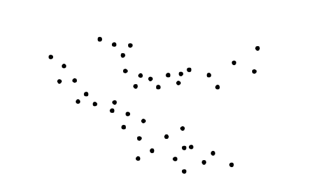
\includegraphics[width=0.25\textwidth]{2}
    \caption{Стрічкові}
\end{figure}
	
	\begin{figure}[h]
    \centering
    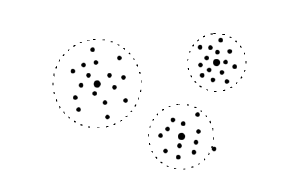
\includegraphics[width=0.25\textwidth]{3}
    \caption{З центром}
\end{figure}

\begin{figure}[h]
    \centering
    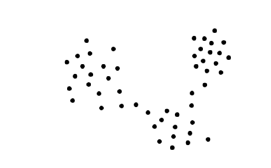
\includegraphics[width=0.25\textwidth]{4}
    \caption{З'єднані перемичками}
\end{figure}
	
	
\begin{figure}[h]
    \centering
    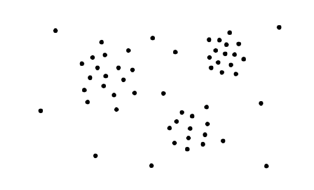
\includegraphics[width=0.25\textwidth]{5}
    \caption{Накладені на шум}
\end{figure}

\begin{figure}[h]
    \centering
    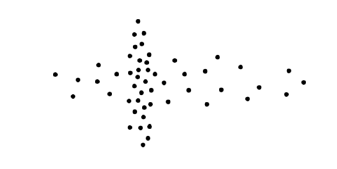
\includegraphics[width=0.25\textwidth]{6}
    \caption{Ті що перетинаються}
\end{figure}

\begin{figure}[h]
    \centering
    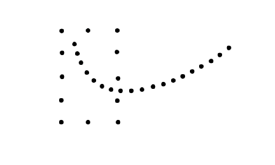
\includegraphics[width=0.25\textwidth]{7}
    \caption{Об'єднані не за схожістю, а за іншими ознаками}
\end{figure}

\begin{figure}[h]
    \centering
    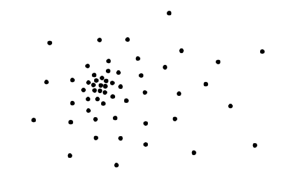
\includegraphics[width=0.25\textwidth]{8}
    \caption{Кластерів не існує}
\end{figure}

\newpage







\chapter{Алгоритми кластеризації}

	\section{Статистичні}
	Статистичні алгоритми побудовані на припущенні, що кластери непогано описуються деяким сімейством ймовірнісних розподілів. Тоді задача кластеризації зводиться до поділу розподілів за кінцевою вибіркою.
	\subsection{EM - алгоритм}
	\textbf{Гіпотеза}(про природу випадковості даних). Об'єкти вибірки  $X^l$ обираються випадковим чином відповідно до їхнього розподілу описуючи розподіл:
	
	$$ p(x) = \sum_{y \in Y}w_y p_y (x), \ \sum_{y \in Y}w_y = 1$$,
	
	де $p_{y}(x)$ - функція густини розподілу кластера $y, w_y$ - невідома апріорна ймовірність появи об'єктів з кластера $y$. Зазвичай коли конкретизують вид розподілу $p_y(x)$, частіше за все обирають сферичні розподіли. Для того, щоб нам було зручно нормувати наші клстери ми припускаємо, що наші кластери мають вигляд еліпсів, які витягнуті вздовж осі x або y. При такому підході оптимальне нормування обирається самим алгоритмом кластеризації, окремо для кожного кластера.\\ \\
	Гіпотеза(про форму кластерів). Об'єкти описуються за допомогою n числових ознак $f_1(x),...,f_n(x), X= R^n $. Кожний кластер $y \in Y$ описується n-мірним гаусівською густиною $p_y(x) = N (x;\mu_y, \sum_{y})$ з центром $ \mu_{y} = (\mu_{y1}, ..., \mu_{yn})$ і діагональною матрицею коваріації $\sum_{y} = diag(\delta_{y1}^2,...,\delta_{yn}^2)$.
	\par EM - алгоритм
	
	\begin{itemize}
		
		\item E - крок	(expectation)\\
		$g_{iy} = P(y|x_i) = \dfrac{w_y p_y(x_i)}{\sum_{z \in Y} w_y p_z(x_i)}, y \in Y, i = 1,...,l;$
		\item M - крок (maximization): \\
			$w_y = \dfrac{1}{l} \sum_{i=1}^{l} g_{iy}, y \in Y;$\\
			$\mu_yi = \dfrac{1}{lw_y} \sum_{i=1}^{l} g_{iy} f_j(x_i), y \in Y, j =1,...,n;$\\
			$\delta_{yj}^{2} = \dfrac{1}{lw_y} \sum_{i=1}^{l} g_{iy}(f_j(x_i) - \mu_{yj})^2, y \in Y,  j =1,...,n; $
			
			\item 
			$y_i = arg \max_{y \in Y} g_{iy}, i=1,...,l;$
	
	
	\end{itemize}
	
	\subsection{k - mean алгоритм}
	Даний алгоритм є спрощеною формою EM - алгоритм. Головна відмінність полягає в тому, що в  ЕМ-алгоритмі кожний об'єкт $x_i$, розподіляється по всім кластерам з ймовірністю $g_{iy} = P \{ y_i=y \}$. В алгоримі k-середніх(k-mean) кожний об'єкт закріплюється за одним кластером.\\ 
	
	 k-mean алгоитрм:

\begin{itemize}
\item	Дослідник визначає кількість кластерів, що необхідно утворити

\item Випадковим чином обирається k спостережень, які на цьому кроці вважаються центрами кластерів

\item Кожне спостереження  $x_i$  «приписується» до одного з n кластерів, відстань до якого найкоротша
Аналог E - кроку: \\
 		$y_i = arg \min_{y \in Y} \varrho (x_i,\mu_y), i=1,..,l;$

\item Розраховується новий центр кожного кластера як елемент, ознаки якого розраховуються як середнє арифметичне ознак об'єктів, що входять у цей кластер
Аналог  M - кроку: \\

 		$\mu_{yj} = \dfrac{\sum_{i=1}^{l} [y_i=y]f_j(x_i)}{\sum_{i=1}^{l}[y_i = y]}, y \in Y, j = 1,...,n;$

\item Відбувається така кількість ітерацій (повторюються кроки 3-4), поки кластерні центри не стануть стійкими (тобто при кожній ітерації в кожному кластері опинятимуться одні й ті самі об'єкти), дисперсія всередині кластера буде мінімізована, а між кластерами — максимізована
	
\end{itemize}	
	
\par Недоліки алгоритму: 
	
\begin{itemize}

  \item  Результат класифікації сильно залежить від випадкових початкових позицій кластерних центрів
\item    Алгоритм чутливий до викидів, які можуть викривлювати середнє
\item     Кількість кластерів повинна бути заздалегідь визначена дослідником

\end{itemize}	
\par 
Існує два "канонічних варіанта"  k-mean. Варіант Болла-Холла[5,110] ми описали попередньо. Варіант МакКіна[5,98] відрізняється тим, що кроки 3 та 4 виконуються в середині одного циклу по об'єктам вибірки. Коли знаходиться об'єкт, що переходить з одного кластера в інший, центри обох кластерів переобчислюються.\par 
K-mean алгоритм дуже чутливий до вибірки початкових наближень центрів. Випадкова ініціалізація на першому кроці може привести до поганої кластеризації. Для формування початкового наближення краще за все виділити  k найбільш віддалених точок вибірки: перші дві точки виділяються по максимуму всіх попарних відстанней, кожна наступна точка обирається так, щоб відстань від неї до найближчої уже виділеної була максимальною. \par 
Кластеризація може виявитись некорекною в тому випадку, якщо спочатку не вгадати правильну кількість кластерів. Зазвичай рекомендують  - провести кластеризацію при різних значеннях k і обрати те, при якому різко покращується кластеризація по заданому функціоналу.
	
	\section{Ієрархічні}
	Ієрархічні алгоритми кластеризації, які також називають таксономією, будують не одне розбиття вибірки на класи, що не перетинаються, а систему вкладених розбиттів. Результатом таксонімії зазвичай представляють у вигляді \textit{дендрограми}. Класичним прикладом такого дерева є є ієрархічна класифікація тварин та рослин. \par
Ієрархічні алгоритми кластеризації розділяють на два основних типи. 
Низхідні алгоритми розбивають вибірку на все більш і більш
дрібні кластери. Більше поширені
агломеративні
або висхідні алгоритми, в яких об'єкти об'єднуються у все більш і більш великі кластери.

   	\subsection{Формула Ланса-Уільямса}
   	Спочатку кожний об'єкт представляє окремий кластер. Для одноелементних кластерів функція відстані визначається наступним чином:  \\
   	$ R ( \{ x \}, \{ x^{'} \} ) = \varrho ( x, x^{'}) $. \par 
   	Потім запускається процес злиття. На кожній ітерації замість пари найближчих кластерів U та V створюється новий кластер $ W = U \cup V $. Відстань від нового кластера W до будь-якого кластера S обчислюється по відстаннях $R(U,V)$, $R(U,S)$ та $R(V,S)$, які на момент обчислення  мають бути відомими: \\
   	$R(U \cup V,S) = \alpha_{u}R(U,S) + \alpha_{v}R(V,S) + \beta R(U,V) + \gamma | R(U,S) - R(V,S)| $, де $\alpha_{u}, \alpha_{v}, \beta, \gamma$ - числоаві параметри. Ця універсальна формула узагальнює майже усі способи визначення відстаней між кластерами.\par 
   	На практиці використовують наступні способи обчислення відстаней $R(W,S)$ між кластерами $W$ та $S$. Для кожного з них існує доведення відповідності формулі Ланса-Уільямса при заданих параметрах[5].
   	\newline
   	
   	\begin{itemize}
   	\item Відстань ближнього сусіда  	\[ R^{n}(W,S) = \min_{w \in W, s \in S} \varrho(w,s); \ \ \ \ \alpha_{u} = \alpha_{v} = \dfrac{1}{2}, \beta = 0, \gamma = - \dfrac{1}{2}\] 

    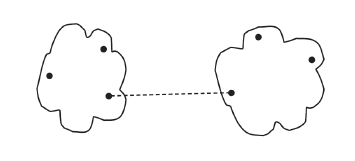
\includegraphics[width=0.25\textwidth]{9}

   	
   		\item Відстань дальнього сусіда  	\[ R^{f}(W,S) = \max_{w \in W, s \in S} \varrho(w,s); \ \ \ \ \alpha_{u} = \alpha_{v} = \dfrac{1}{2}, \beta = 0, \gamma = - \dfrac{1}{2}\] 
   	
    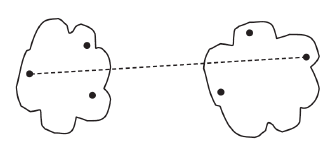
\includegraphics[width=0.25\textwidth]{10}

   		
   		   \item Середня відстань  	\[ R^{c}(W,S) = \dfrac{1}{|W||S|} \sum_{w \in W} \sum_{s \in S} \varrho(w,s); \ \ \ \ \alpha_{u} = \dfrac{|U|}{|W|} \alpha_{v} = \dfrac{|V|}{|W|}, \beta = \gamma = 0\] 
   		   


    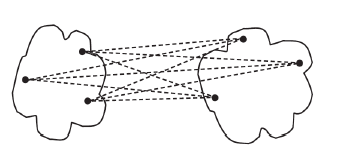
\includegraphics[width=0.25\textwidth]{11}

   		   \item Відстань між центрами 
   		   		\[ R^{m}(W,S) = \varrho^{2} ( \sum_{w \in W} \dfrac{w}{|W|} \sum_{s \in S} \dfrac{s}{|S|} )\ \ \ \ \alpha_{u} = \dfrac{|U|}{|W|} \alpha_{v} = \dfrac{|V|}{|W|}, \beta = - \alpha_{u} \alpha_{v}, \gamma = 0\] 

   		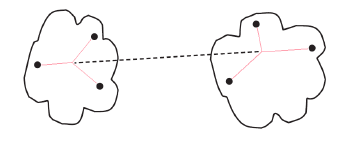
\includegraphics[width=0.25\textwidth]{12}
   		
    
   		   		
   		   		  \item Відстань Уорда 
   		   		\[ R^{u}(W,S) = \dfrac{|S||W|}{|S|+|W|} \varrho^{2} ( \sum_{w \in W} \dfrac{w}{|W|} \sum_{s \in S} \dfrac{s}{|S|} ) \] \[\alpha_{u} = \dfrac{|S|+|U|}{|S| + |W|} \alpha_{v} = \dfrac{|S|+|V|}{|S|+|W|}, \\ \beta = \dfrac{-|S|}{|S|+|W|}, \gamma = 0\] 
   		   		
   		   		

   	\end{itemize}
\par 
Алгоритм Ланса-Уільямса:  \\
\begin{itemize}

\item Спочатку усі кластери одноелементні  $ t:=1;  C_t = \big\{ \{ x_1 \} ,..., \{ x_l \} \big\}; $ 
\item Для усіх $t = 2, ..., l$(t - номер ітерації)
\item Знайти в  $C_{t-1}$ два найближчиш кластера: \\ $(U,V) = arg \min_{U \ne V}R(U,V);$\\
$R_t = R(U,V);$

\item Злити в один кластер: \\
$W = U \cup V;$\\
$ C_t = C_{t-1} \cup {W} \ {U,V}$
\item Для всіх $S \in C_t$ \\ обрахувати $R(W,S)$ по формулі Ланса-Уільямса.
\end{itemize}
\par 
	Деякі відстанні мають характеристику розтягу. По мірі того, як кластер росте, то відстань від нього до других кластерів також росте, так ніби простір навколо кластера розтягується. Характеристика розтягу є бажаною, так як вона сприяє більш чіткому відділеню кластерів. З іншого боку, при сильно великих розтягах можна знайти кластери там, де їх не було. Розтягуючими є відстані: $R^f \ , R^u$.\par 
	
	Деякі відстані, навпаки,  характерезуються стискання. По мірі того, як кластерна відстань зростає від інших кластерів вона зменшується, і здається, що простір навколо кластера стискається. Природня кластеризація при цьому "розмивається". Відстань ближнього сусіда $R^n$ є стискаючим. \par 
	Характеристика стискання та розтягу визначається через відношення $R_t/ \varrho(\mu_U, \mu_V)$, де $R_t = R(U,V)$ - відстань між ближніми кластерами, що об'єднуються на кроці t, $\mu_U, \mu_V$ - центри цих кластерів. Якщо це відношення на кожному кроці більше одиниці, то $R$ є розтягуючим, якщо менше - стискаючим. Є такі відношення які є ні стисканням ні розтягом $R^c, R^m$. Про них говорять, що вони зберігають метрику простору.\par 
	на практиці використовують гнучку відстань, яка являє собою компроміс між методами ближнього сусіда, дальнього сусіда та середньої відстані. Вона визначається одним параметром  $\beta$ замість чотирьох: \\
	$\alpha_U = \alpha_V = (1-\beta)/2, \gamma = 0, \beta < 1$.
	\\
	Гнучка відстань є стискаючим при $\beta > 0$ і  розтягуючим при $\beta < 0$. Стандартна рекомендація :  $\beta = -0.25$[6].


\par Достатки та недоліки: 
	Точної відповіді на питання, який алгоритм кластеризації підходить найкраще, не існує. Кожна, із вище перерахованих відстаней, має свої переваги та недоліки в контексті конкретної задачі. \par 
	Метод найближчого сусіда характеризується ланцюговим ефектом, коли незалежно від форми кластера до нього приєднуються найближчі об'єкти. В деяких випадках це приводить до того, що кластири "відрощують щупальці". В залежності від задачі ця характеристика може бути як корисною так і поганою. Цей метод найкраще підходить для виділеня стрічкових кластерів.
	\par 
	Метод дальнього сусіда ланцюгового ефекту не має, але на ранньому етапі він може об'єднати несхожі групи. \par 
	Відстань між центрами мас не монотонне та не руктивне, тому воно на практиці майже не застосовується, хоча інтуєтивно воно здається золотою серединою у виборі алгоритму. \par 
	Метод Уорда експерементально виявився найкращим з усіх перерахованих методі[5]. Він найкраще розбиває дані на інтуєтивні кластери.
	\section{Графові}
	Великий клас алгоритмів кластеризації базується на предствленні вибірки у вигляді графа. Вершина графа відповідає об'єкту вибірки, а ребара - попарні відстані між об'єктами $ \varrho_{ij} = \varrho(x_i, x_j)$. \par 
	Перевагою графових алгоритмів кластеризації є наглядність, простота реалізації, можливість оптимізовувати алгоритм, спираючись на прості геометричні міркування. 
	
		\subsection{Алгоритм знаходження зв'язних компонентів}
		Задається параметр $R$ і в графі видаляяються ребра $(i,j)$, для яких $\varrho_{ij} > R$. З'єднаними залишаються лиш найближчі пари об'єктів. Ідея алгоритма полягає в тому, щоб підібрати таке значення $R \in [min \ \varrho_{ij}, max \ \varrho_{ij}]$, при якому граф розбивається на декілька компонентів зв'язності. Знайдені зв'язні компоненти - і є кластери. \par 
		\textit{Компонентою зв'язності} графа називається підмножина його вершин, в якій будь - які дві вершини можна з'єднати шляхом. Для пошуку зв'язних компонентів можна використовувати усім відомий BFS (алгоритм Дейкстри) або DFS. \par
		Для вибору параметра $R$ рекомендують побудувати гістограму розподілу попарних відстаней $\varrho_{ij}$. В задачах з вираженою кластерною структурою ця гістограма має два чітких піка: зона найбільших внутрішніх міжкласових відстаней та найменших внутрішніх міжкласових відстаней. Параметр $R$ задається як відстань, що відповідає точці мінімума між цими піками.
		Недоліки алгориму:
		\begin{itemize}
			
			\item Обмежена область використання. Алгоритм знаходження зв'язних компонентів найбільше підходить для виділення кластерів класу концентрації чи стрічок. Наявність розрідженого фонe чи "вузьких перемичок" між кластерами призведе до некоректної кластеризації. 
			
			\item Погана керованість числом кластерів. Для багатьох задач зручніше не задавати параметр $R$, а вказувати кількість кластерів. Керувати числом кластерів за допомогою параметра $R$ важко. Доводиться вирішувати цю задачу декілька раз при різних значеннях параметра $R$,що негативно впливає на чис вирішення задачі.
		
		\end{itemize}
		
		\subsection{Алгоритм знаходження найкоротшого незамкненого шляху}
		
		Алгоритм будує гарф з $l- 1$ ребер так, щоб вони з'єднували всі $l$ точок і мали найменшу сумарну довжину. Такий граф називається \textit{найкоротшим незамненем шляхом}, або остове дерево. \par 
		На відмінно від попереднього алгоритму, тут число кластерів $K$ задається як вхідний параметр. 
		Недоліки алгориму:
		\begin{itemize}
		
			\item 	Обмежена область використання.  Наявність розрідженого фонe чи "вузьких перемичок" між кластерами призведе до некоректної кластеризації. 
			
			\item Для побудови найкоротшого незамкнутого шляху потрібно виконати $O(l^3)$ операцій.
		
		
		\end{itemize}
		
		
	 
	 
\chapter{Практична частина}
В якості практичної частини розглянемо побудову пошукової системи для форуму. Коли користувач буде шукати на нашому форумі інформацію, наша пошукова система, скоріш за все видасть йому правильну відповідь на постевлене запитання, якщо така існує - в іншому випадку вона виведе найбільш схожу відповідь.\par 
Для вирішення цієї задачі ми і будемо використовувати кластеризацію. Для реалізації ціє ідеї нам потрібно буде виконати наступні дії:

\begin{enumerate}
\item Зробити лексичний аналіз тексту та розбити його на лексеми
\item Відкинути слова, що зустрічаються дуже часто і не допомагають знаходити релевантні повідомлення
\item Відкинути слова, що зустрічаються дуже рідко, і наврядчи зустрінуться в наступних повідемленнях
\item Обрахувати  TF-IDF з урахуванням усього корпусу тексту.
\item Виділити характерні ознаки з кожного повідомлення і зберегти його в вигляді асоційованого масиву з повідомленням 
\item Побудувати кластери з цих векторів
\item Визначити кластер до якого відноситься повідомлення
\item Обрати з цього кластеру кілька повідомлень, що маю достатню міру схожості з повідомленням. Це підвищить різноманіття видачі.
\end{enumerate}

Для реалізації програми ми будемо використовувати бібліотеку SciKit.

\par 
Для перетворення тексту в вектор числових значення будемо використовувати  інвертований індекс. При використанні цього підходу перше з чим ми стикаємось -  попередня обробка даних. Для підрахунку використаємо метод CountVectorizer з бібліотеки SciKit. 

\begin{lstlisting}[frame=single]  % Start your code-block

CountVectorizer(analyzer= 'word', binary= False,
 charset = None,
charset_error= None, decode_error='strict',
dtype= <class 'numpy.int64'>, encoding = 'utf-8',
input='content',
lowercase= True, max_df=l.O, max_features=None, min_df=l,
ngram_range=(l, 1), preprocessor=None, stop_words=None,
strip_accents= None, token_pattern=' (?u)\\b\\w\\w+\\b',
tokenizer=None, vocabulary= None)
\end{lstlisting}

Для обрахунку міри схожості між векторами будемо обраховувати, як відстань між нормованими векторами.

\begin{lstlisting}[frame=single]  
>>> def dist_norm(vl, v2):
vl_normalized = vl/sp.linalg.norm(vl.toarray())
v2_normalized = v2/sp.linalg.norm(v2.toarray())
delta = vl_normalized - v2_normalized
return sp.linalg.norm(delta.toarray())
\end{lstlisting}
\par 
Наступним кроком для підготовки тексту є видалення так званих "стоп-слів". Для цього нам необхідно передати відповідний параметр в наш CounteVectorizer.

\begin{lstlisting}[frame=single]  
>>> vectorizer = CountVectorizer(min_df = l, stop_words='english')
\end{lstlisting}
Якщо параметр stop \_ words = english, то в цей список буде складатися 318 англійських слів.

\begin{lstlisting}[frame=single]  
>>> sorted(vectorizer.get_stop_words()) (0:20)
['a','about','above','across','after','afterwards','again',
'against','all','almost','alone','along','already','also',
'although','always','am','among','amongst','amoungst']
\end{lstlisting}

Наступним етапом обробки даних буде стемінг. Стемінг - це процес скорочення слова до основи шляхом відкидання допоміжних частин, таких як закінчення чи суфікс. Результати стемінгу іноді дуже схожі на визначення кореня слова, але його алгоритми базуються на інших принципах. Тому слово після обробки алгоритмом стемінгу (стематизації) може відрізнятися від морфологічного кореня слова.
\\

Для роботи з стемером ми будемо використовувати бібліотеку NLTK. З цього пакету будемо використовувати SnowballStemmer. \\ 

Також для узагальнення концепції стоп-слів, для часто вживаних слів, ми будемо використовувати TF-IDF(term frequency - inverse document frequency). Для цього ми використаємо TdfidVectorizer з пакету SciKit. \\


Для перевірки реалізації нашої системи будемо використовувати один із стандартних, для машинного навчання, набір даних 20newsgroup, який складається з 18826 повідомлень та із 20 новинних груп за різними тематиками. Увесь код реалізації можна знайти у додатку до даної роботи.

\newpage
\likechapter{Висновки}
У цій роботі ми розглянули основні алгоритми кластеризації інформації, а також побудували систему, яка здатна обробити зашумлений текст в компактне векторне представлення, яке ми вдало кластеризували. За допомогою кластеризації наша система може злегкістю видавати релевантні відповіді користувачу, що ми і прагнули зробити.
\newpage

\begin{thebibliography}{9}
\bibitem{voron}
Воронцов К.В. Алгоритмы кластеризации и многомерного шкалирования. Курс лекцій. МГУ, 2007.

\bibitem{jain} 
Jain A., Murty M., Flynn P. Data Clustering: A Review.  ACM Computing Surveys. 1999. Vol. 31, no. 3.
 
\bibitem{mandel} 
 Мандель І. Д. Кластерний аналіз - М.: Фінанси та Статистика, 1998 

\bibitem{wiliams} 
 Уілліамс У. Т., Ланс Д. Н. Методи ієрархічної класифікації  Статистичні методи для ЕОМ  Під ред. М. Б. Малюта.  М .: Наука, 1986. С. 269-301.
\end{thebibliography}


\newpage
\likechapter{Додаток}

\end{document}
